\usetikzlibrary{arrows}
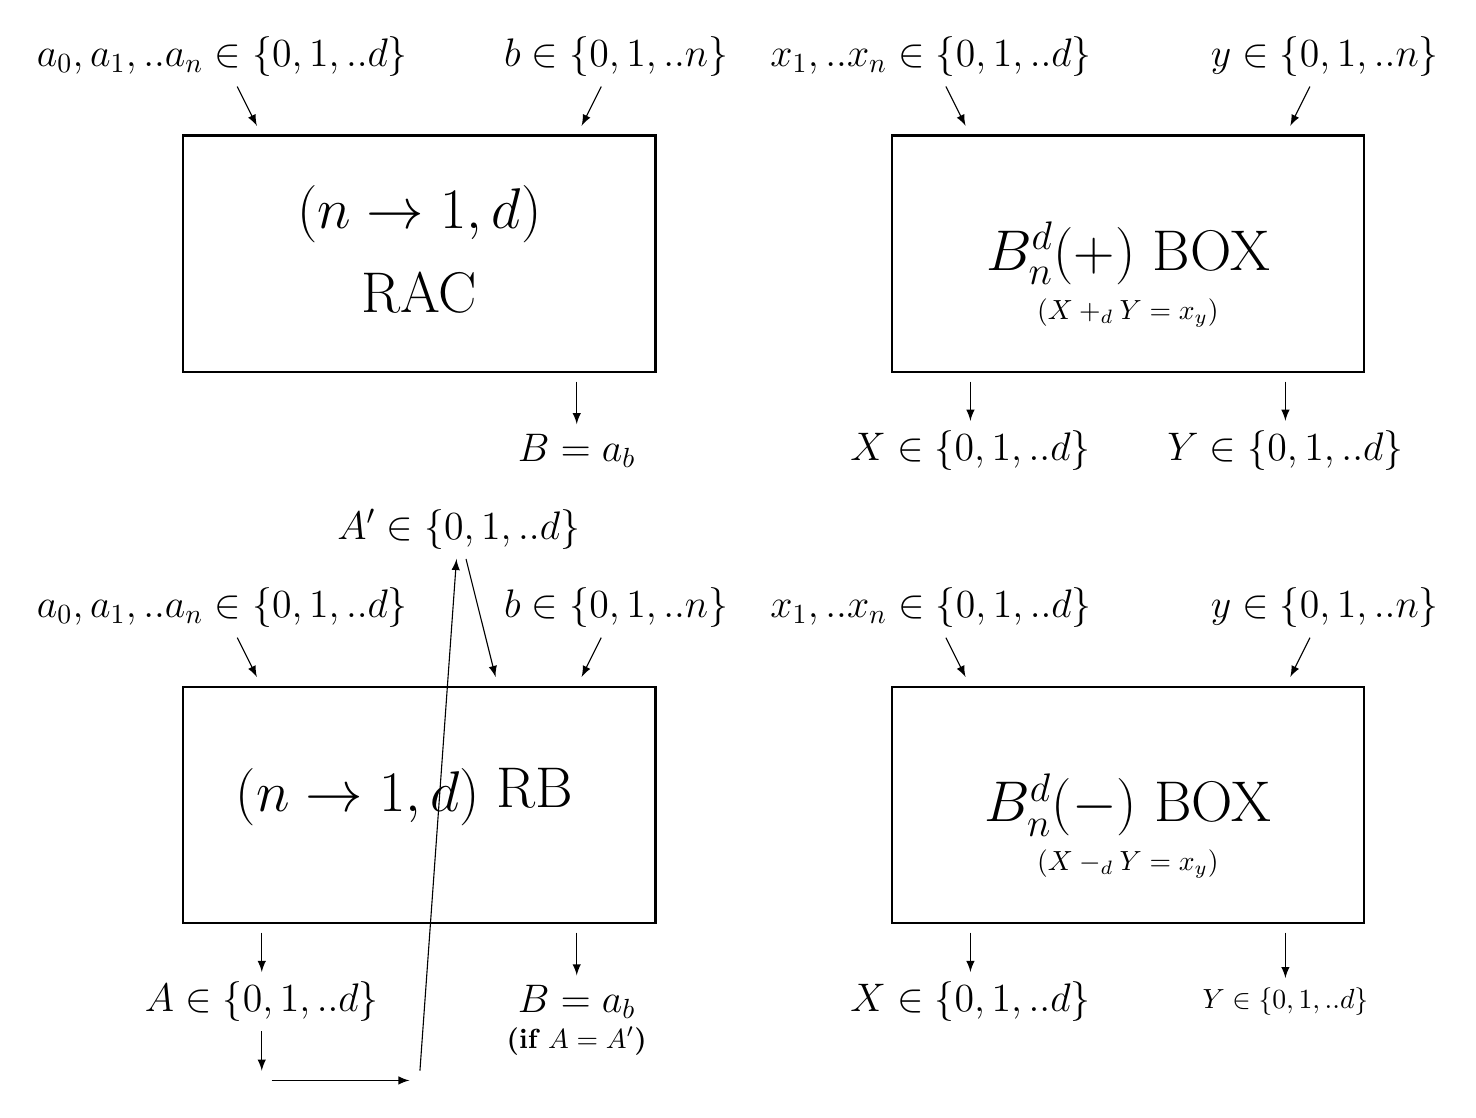
\begin{tikzpicture}

\draw[thick]  (-7.5,6) rectangle (-1.5,3);
\draw[thick]  (1.5,6) rectangle (7.5,3);

\draw[thick]  (-7.5,-1) rectangle (-1.5,-4);
\draw[thick]  (1.5,-1) rectangle (7.5,-4);
\node (v1) at (-7,7) {\Large $a_0,a_1,..a_n\in\{0,1,..d\}$};
\node (v2) at (-6.5,6) {};
\node (v3) at (-2,7) {\Large $b\in\{0,1,..n\}$};
\node (v4) at (-2.5,6) {};
\node (v9) at (-2.5,3) {};
\node (v10) at (-2.5,2) {\Large $B=a_b$};
\node (v5) at (2,7) {\Large $x_1,..x_n\in\{0,1,..d\}$};
\node (v6) at (2.5,6) {};
\node (v7) at (7,7) {\Large $y\in\{0,1,..n\}$};
\node (v8) at (6.5,6) {};
\node (v13) at (6.5,3) {};
\node (v14) at (6.5,2) {\Large $Y\in\{0,1,..d\}$};
\node (v11) at (2.5,3) {};
\node (v12) at (2.5,2) {\Large $X\in\{0,1,..d\}$};
\node (v15) at (-7,0) {\Large $a_0,a_1,..a_n\in\{0,1,..d\}$};
\node (v16) at (-6.5,-1) {};
\node (v19) at (-2,0) {\Large $b\in\{0,1,..n\}$};
\node (v20) at (-2.5,-1) {};
\node (v17) at (-4,1) {\Large $A'\in\{0,1,..d\}$};
\node (v18) at (-3.5,-1) {};
\node (v21) at (-6.5,-4) {};
\node (v22) at (-6.5,-5) {\Large $A\in\{0,1,..d\}$};
\node (v23) at (-2.5,-4) {};
\node (v24) at (-2.5,-5) {\Large $B=a_b$};
\draw [o-*, -latex] (v1) edge (v2);
\draw [o-*, -latex] (v3) edge (v4);
\draw [o-*, -latex] (v5) edge (v6);
\draw [o-*, -latex] (v7) edge (v8);
\draw [o-*, -latex] (v9) edge (v10);
\draw [o-*, -latex] (v11) edge (v12);
\draw [o-*, -latex] (v13) edge (v14);
\draw [o-*, -latex] (v15) edge (v16);
\draw [o-*, -latex] (v17) edge (v18);
\draw [o-*, -latex] (v19) edge (v20);
\draw [o-*, -latex] (v21) edge (v22);
\draw [o-*, -latex] (v23) edge (v24);
\node (v25) at (-6.5,-6) {};
\node (v26) at (-4.5,-6) {};
\draw [o-*,  -latex, -latex] (v22) edge (v25);
\draw [o-*,  -latex, -latex] (v25) edge (v26);
\draw [o-*,  -latex, -latex] (v26) edge (v17);
\node at (-2.5,-5.5) {\textbf{(if $A=A'$)}};
\node at (-4.5,5) {\huge $(n\rightarrow1,d)$};
\node at (-4.5,4) {\huge RAC};
\node at (4.5,4.5) {\huge $B_n^d(+)$ BOX};
\node at (-5.2772,-2.4003) {\huge $(n\rightarrow1,d)$};
\node at (-3.0276,-2.2791) {\huge RB};
\node at (4.5,3.75) {$(X+_d Y=x_y)$};
\node (v27) at (2,0) {\Large $x_1,..x_n\in\{0,1,..d\}$};
\node (v28) at (2.5,-1) {};
\node (v29) at (7,0) {\Large $y\in\{0,1,..n\}$};
\node (v30) at (6.5,-1) {};
\node (v31) at (2.5,-4) {};
\node (v32) at (2.5,-5) {\Large $X\in\{0,1,..d\}$};
\node (v33) at (6.5,-4) {};
\node (v34) at (6.5,-5) {$Y\in\{0,1,..d\}$};
\draw [-latex] (v27) edge (v28);
\draw [-latex] (v29) edge (v30);
\draw [-latex] (v31) edge (v32);
\draw [-latex] (v33) edge (v34);
\node at (4.5,-2.5) {\huge $B_n^d(-)$ BOX};
\node at (4.5,-3.25) {$(X-_d Y=x_y)$};
\end{tikzpicture} 